\documentclass[]{article}
\usepackage[italian]{babel}
\usepackage[margin=3mm,a3paper]{geometry}
\usepackage{float}
\usepackage[dvipsnames]{xcolor}
\usepackage{multicol}
\usepackage{color,soul}
\usepackage{graphicx}
\usepackage{amsmath}
\usepackage{amssymb}
\usepackage{bm}
\usepackage{cancel}
\usepackage{subcaption}
\usepackage{wrapfig,lipsum}
\usepackage{tikz}
\usepackage{enumitem}
\usepackage{mathtools}
\usepackage{colortbl} % for cell color
\usepackage{graphbox}
\usepackage{emoji}


\setlist[itemize]{left=0pt}


\usepackage{titlesec}
%\titleformat*{\section}{\normalsize\bfseries}
\titlespacing*{\section}{0pt}{10pt}{10pt}
\titlespacing*{\paragraph}{0pt}{0pt}{3pt}

% Horizontal line before ssection
\titleformat{\section}
{
	\ifnum \value{section}>1
		\ifnum \value{section}=5
			% Do nothing if section number is 5
		\else
			\vbox{\rule{\linewidth}{0.8pt}}
		\fi
	\fi
	\Large\bfseries
}
{\thesection.}
{0.5em}
{}


%\frenchspacing % end of sentence space is not different from the normal inter-word spacing

\setlength{\columnseprule}{0.3pt}
\setlength{\columnsep}{0.5cm}




% ---------- NEW COMMANDS ----------
\newcommand*\circled[1]{\tikz[baseline=(char.base)]{\node[shape=circle,draw,inner sep=2pt] (char) {#1};}} % Circled number

\newcommand{\R}{\mathbb{R}}
% ----------------------------------



\graphicspath{ {images/} }


\begin{document}
	
	\setlength{\abovedisplayskip}{1pt}
	\setlength{\belowdisplayskip}{1pt}
	\setlength{\abovedisplayshortskip}{1pt}
	\setlength{\belowdisplayshortskip}{1pt}
	
	\setlength\parindent{0pt}
	%\setcounter{secnumdepth}{0}
	
\begin{multicols*}{2}

\section{Denavit-Hartenberg}

\vspace*{-15pt}
\begin{figure}[H]
	\hspace*{10pt}
	\begin{subfigure}{0.23\columnwidth}
		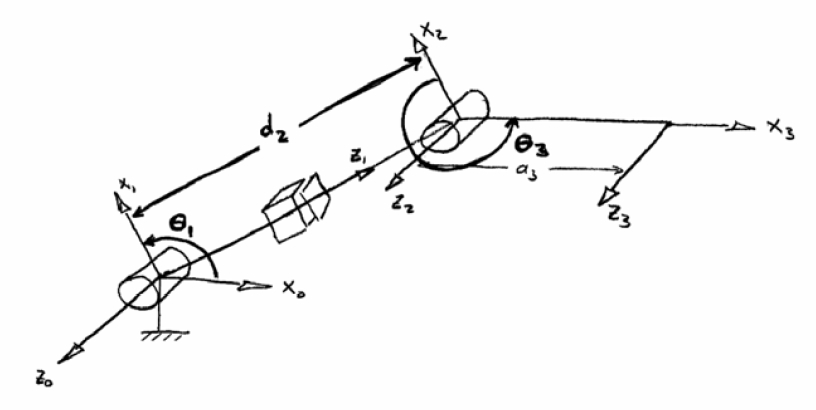
\includegraphics[align=c,angle=90,origin=c,width=\linewidth]{images/dh2}
	\end{subfigure}
%	\hspace*{pt}
	\begin{subfigure}{\columnwidth}
		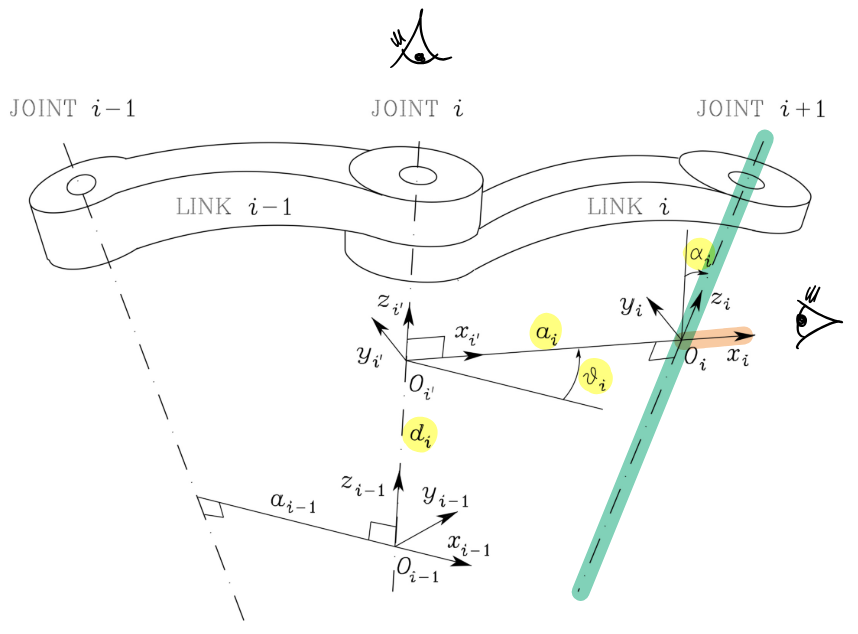
\includegraphics[align=c,width=0.7\linewidth]{images/dh}
	\end{subfigure}
\end{figure}
%\begin{figure}[H]
%	\centering
%	\includegraphics[width=0.6\linewidth]{images/kinematics_9}
%\end{figure}

Il sistema di riferimento $\mathcal{R}_i$ solidale con $\textit{LINK}_i$ viene definito secondo le seguenti regole:\\

\circled{1} \textbf{Asse $z_i$ e origine $O_i$}
\begin{itemize}
	\item \colorbox{Green}{\textbf{L’asse} $\boldsymbol{z_i}$} è posto lungo l’asse di movimento di $g_{i+1}$ (asse di rotazione o di traslazione a seconda del tipo di giunto)
	\item \textbf{L’origine} $\boldsymbol{O_i}$ è posta all’intersezione di $z_i$ con la normale comune (\textit{common normal}) fra gli assi $z_{i-1}$ e $z_i$.
	La normale comune è quella retta perpendicolare ad entrambi gli assi (nota: entrambi angoli retti nella figura)
	\item \textbf{Casi particolari}:
	\vspace*{-3pt}
	\begin{itemize}
		\item $\boldsymbol{\mathcal{R}_0}$: origine $O_0$ e $x_0$ possono essere fissati a piacimento (solo $z_0$ univocamente definito).
%		qua è univocamente definita solo la direzione di $z_0$, data dall’asse di movimento di $g_1$; l’origine $O_0$ e $x_0$ possono essere fissati a piacimento
		\item $\boldsymbol{\mathcal{R}_n}$: $\nexists \ g_{n+1} \implies z_n, \ O_n$ non univocamente definiti. Per consuetudine: origine nel centro della pinza e $z_n$ coincidente a a $z_{n-1}$ (visto che tipicamente l'ultimo giunto è rotoidale).
	\end{itemize}
\end{itemize}
\vspace*{5pt}

\circled{2} \textbf{Asse $x_i$ e $y_i$}
\begin{itemize}
	\item \colorbox{YellowOrange}{\textbf{L’asse $\boldsymbol{x_i}$}} è fissato lungo la normale comune fra gli assi $z_{i-1}$ e $z_i$
	\begin{itemize}
		\item Se $z_{i-1}$ e $z_i$ si intersecano $\implies$ direzione di $x_i$ ($\perp z_i$) è arbitraria
		%l’origine di $\mathcal{R}_i$ coincide con il loro punto di intersezione e la direzione di $x_i$ (ortogonale a $z_i$) è arbitraria
		\item se $z_{i-1}$ e $z_i$ sono paralleli $\implies$ origine arbitraria, $x_i$ nel piano normale a $z_{i-1}$ e $z_i$ con direzione e verso arbitrari.
	\end{itemize}
	\item \textbf{L’asse $\boldsymbol{y_i}$} completa la terna destrorsa ($j = k\times i$)
\end{itemize}
\vspace*{5pt}

\circled{3} \textbf{Sistema di riferimento intermedio}\\[5pt]
$z_{i'}$ diretto lungo $z_{i-1}$ $|$ $O_{i'}$ posta all’intersezione di $z_{i-1}$ con la normale comune fra $z_{i-1}$ e $z_i$ $|$ $x_{i'}$ diretto lungo la normale comune fra $z_{i-1}$ e $z_i$ (come $x_i$)

\vspace*{10pt}

\setlength{\fboxsep}{7pt} % Adjust the padding as needed
\fbox{
\begin{minipage}{0.93\columnwidth}
	\begin{itemize}
		\item $\boldsymbol{d_i} \rightarrow$ \textbf{link offset}: coordinata di $O_{i'}$ lungo $z_{i-1}$
		\item $\boldsymbol{\theta_i} \rightarrow$ \textbf{joint angle}: angolo di rotazione da $x_{i-1}$ a $x_i$ attorno all'asse $z_{i'}$ (positivo quando la rotazione è anti-oraria)
		\item $\boldsymbol{a_i} \rightarrow$ \textbf{link length}: distanza (con segno) fra $O_i$ e $O_{i'}$
		\item $\boldsymbol{\alpha_i} \rightarrow$ \textbf{link twist}: angolo di rotazione da $z_{i-1}$ a $z_i$ attorno all'asse $x_i$ (positivo quando la rotazione è anti-oraria)
	\end{itemize}

$$
{}^{i-1}\mathbf{T}_{i}(q_i)
=
\begin{bmatrix}
	c\theta_i & -s\theta_ic\alpha_i & s\theta_is\alpha_i & a_ic\theta_i \\
	s\theta_i & c\theta_ic\alpha_i & -c\theta_is\alpha_i & a_is\theta_i \\
	0 & s\alpha_i & c\alpha_i & d_i \\
	0 & 0 & 0 & 1
\end{bmatrix}
$$
\end{minipage}
}

\vspace*{7pt}
\textbf{Trigonometric inequalities}:
$$
c_{12} + s_{12} = c_{1-2}
\qquad
c_{12} - s_{12} = c_{1+2}
\qquad
s_1c_2 - c_1s_2 = s_{1-2}
\qquad
s_1c_2 + c_1s_2 = s_{1+2}
$$

\vspace*{10pt}
\textbf{Tips}:
\begin{align*}
a_i &\rightarrow
\begin{cases}
\ z_{i-1} \overset{\text{dist.}}{\longleftrightarrow} z_i \quad \text{along } x_i
%\quad
%> 0 \textit{se concorde} \mathcal{i}_i, <0 \textit{se discorde}
\end{cases}\\
%\text{\small length of common normal, > 0 }\\
%
\alpha_i &\rightarrow
\begin{cases}
\ z_{i-1} \overset{\angle}{\longrightarrow} z_i \quad \text{around } x_i
\end{cases}\\
%
d_i &\rightarrow
\begin{cases}
\ x_{i-1} \overset{\text{dist.}}{\longleftrightarrow} x_i \quad \text{along } z_{i-1}
\end{cases}\\
%
\theta_i &\rightarrow
\begin{cases}
\ x_{i-1} \overset{\angle}{\longrightarrow} x_i \quad \text{around } z_{i-1}
\end{cases}
\end{align*}

\begin{textblock}{5}(5.8,-0.9)
	\small
	$\bm{d}$ \textbf{e} $\bm{a}$ \textbf{sono con segno!}\\
	Relativ. ad "along":\\[5pt]
%	$
%	\begin{cases}
%	$> 0$ \ \text{se concorde} \\
%	$< 0$ \ \text{se discorde}
%	\end{cases}
%	$
	$> 0$ se concorde \\
	$< 0$ se discorde
\end{textblock}
	
\vspace*{-15pt}

\section{Differential Kinematics}

\subsection{Geometric Jacobian}
\vspace*{5pt}
\begin{align*}
	\text{i-th column of } \bm{J} \text{:} \qquad
	\begin{bmatrix}
		\bm{J}_{p,i} \\
		\bm{J}_{o,i}
	\end{bmatrix}
	=
	\begin{cases}
		\begin{bmatrix}
			\bm{z}_{i-1} \\
			\bm{0}
		\end{bmatrix}
		& \textit{for a \textbf{prismatic} joint}
		\vspace*{5pt}
		\\
		\begin{bmatrix}
			\bm{z}_{i-1} \times (\bm{p} - \bm{p}_{i-1}) \\
			\bm{z}_{i-1} 
		\end{bmatrix}
		& \textit{for a \textbf{revolute} joint}
	\end{cases}
\end{align*}

\vspace*{5pt}
%\begin{itemize}
%	\item $\bm{z}_{i-1} = 3^{rd} \text{ column of } {}^0\bm{T}_{i-1} = {}^0\bm{T}_{1} \cdots {}^{i-2}\bm{T}_{i-1}$.
%	\item $\bm{p} = \text{first 3 elements of the last column of } {}^0\bm{T}_n = {}^0\bm{T}_{1} \cdots {}^{n-1}\bm{T}_{}$
%	\item $\bm{p}_{i-1} = \text{first 3 elements of the last column of } {}^0\bm{T}_{i-1} = {}^0\bm{T}_{1} \cdots {}^{i-2}\bm{T}_{i-1}$
%\end{itemize}

\vspace*{8pt}
$$
\begin{bmatrix}0 \\ 0 \\ 1\end{bmatrix}
\times
\begin{bmatrix}x \\ y \\ z\end{bmatrix}
=
\begin{bmatrix}-y \\ x \\ 0\end{bmatrix}
$$


\vspace*{8pt}
\textit{E.g. planar RRR}
$$
J(q)
=
\begin{bmatrix}
	z_0 \times (p - p_0) & z_1 \times (p - p_1) & z_2 \times (p - p_2) \\
	z_0 & z_1 & z_2
\end{bmatrix}
\qquad
\textit{here } \ c_{12} = c(\theta_1+\theta_2)
$$

\newcolumn
\vspace*{-18pt}
\begin{equation*}  
	{}^0T_0
	=
	\begin{bmatrix}
		1 & 0 & \cellcolor{cyan}0 & \cellcolor{yellow}0 \\
		0 & 1 & \cellcolor{cyan}0 & \cellcolor{yellow}0 \\
		0 & 0 & \cellcolor{cyan}1 & \cellcolor{yellow}0 \\
		0 & 0 & 0 & 1 \\
	\end{bmatrix}
	\implies
	\colorbox{cyan}{$z_0$}
	=
	\begin{bmatrix}
		0 \\ 0 \\ 1
	\end{bmatrix}
	\ , \
	\colorbox{yellow}{$p_0$}
	=
	\begin{bmatrix}
		0 \\ 0 \\ 0
	\end{bmatrix}
%	\parbox[position]{4em}{\textbf{N.B.} this is always like this !}
\end{equation*}

\begin{equation*}
	{}^0T_1
	=
	\begin{bmatrix}
		c_1 & -s_1 & \cellcolor{cyan}0 & \cellcolor{yellow}l_1 c_1 \\
		s_1 & c_1 & \cellcolor{cyan}0 & \cellcolor{yellow}l_1 s_1 \\
		0 & 0 & \cellcolor{cyan}1 & \cellcolor{yellow}0 \\
		0 & 0 & 0 & 1 \\
	\end{bmatrix}
	\implies
	\colorbox{cyan}{$z_1$}
	=
	\begin{bmatrix}
		0 \\ 0 \\ 1
	\end{bmatrix}
	\ , \
	\colorbox{yellow}{$p_1$}
	=
	\begin{bmatrix}
		l_1 c_1 \\ l_1 s_1 \\ 0
	\end{bmatrix}
\end{equation*}

%$$
%	\cdots {}^0T_2 = {}^0T_1 {}^1T_2 = \cdots
%$$

\begin{equation*}
	{}^0T_2
	=
	{}^0T_1 {}^1T_2
	=
	\begin{bmatrix}
		c_{12} & -s_{12} & \cellcolor{cyan}0 & \cellcolor{yellow}l_1 c_1 + l_2c_{12}\\
		s_{12} & c_{12} & \cellcolor{cyan}0 & \cellcolor{yellow}l_1 s_1 + l_2s_{12}\\
		0 & 0 & \cellcolor{cyan}1 & \cellcolor{yellow}0 \\
		0 & 0 & 0 & 1 \\
	\end{bmatrix}
	\implies
	\colorbox{cyan}{$z_2$}
	=
	\begin{bmatrix}
		0 \\ 0 \\ 1
	\end{bmatrix}
	\ , \
	\colorbox{yellow}{$p_2$}
	=
	\begin{bmatrix}
		l_1 c_1 + l_2c_{12} \\ l_1 s_1 + l_2s_{12} \\ 0
	\end{bmatrix}
\end{equation*}

\begin{equation*}
	{}^0T_3
	=
	\begin{bmatrix}
		c_{123} & -s_{123} & 0 & \cellcolor{yellow}l_1 c_1 + l_2c_{12} + l_3c_{123}\\
		s_{123} & c_{123} & 0 & \cellcolor{yellow}l_1 s_1 + l_2s_{12} + l_3s_{123}\\
		0 & 0 & 1 & \cellcolor{yellow}0 \\
		0 & 0 & 0 & 1 \\
	\end{bmatrix}
	\implies
	\colorbox{yellow}{$p$}
	=
	\begin{bmatrix}
		l_1 c_1 + l_2c_{12} + l_3c_{123} \\ l_1 s_1 + l_2s_{12} + l_3s_{123} \\ 0
	\end{bmatrix}
\end{equation*}





\subsection{Analytical Jacobian}

\begin{gather*}
\dot{\bm{x}}
=
\begin{bmatrix} \dot{\bm{p}} \\ \dot{\bm{\phi}}\end{bmatrix}
=
\frac{d\bm{x}}{dt}
=
\underbrace{\frac{\partial\bm{x}}{\partial \bm{q}}}_{\bm{J}_A(\bm{q})}
\underbrace{\frac{d\bm{q}}{d t}}_{\dot{\bm{q}}}
=
\bm{J}_A(\bm{q})\dot{\bm{q}}
\quad \qquad
\bm{J}(\bm{q})
=
\begin{bmatrix}
	\bm{I} & \bm{0} \\
	\bm{0} & \bm{T}(\bm{\phi})
\end{bmatrix}
\bm{J}_A(\bm{q})
%\qquad
%\parbox[position]{6em}{$T(\phi)$ depends on the attitude represent.}
\end{gather*}


\vspace*{-5pt}
\subsection{Inverse differential kinematics}
\begin{equation*}
\begin{cases}
\text{minimize} & \quad g(\dot{\bm{q}}) = \frac{1}{2} \dot{\bm{q}}^T \bm{W} \dot{\bm{q}} \\
\text{subject to} & \quad \bm{v} = \bm{J}(\bm{q})\bm{\dot{q}}
\end{cases}
\quad 
\overset{\bm{W} = \bm{I}}{\iff}
%\xLeftrightarrow{\bm{W} = \bm{I}}
\quad
\dot{\bm{q}} = \bm{J}^{\dagger}(\bm{q})\bm{v}
\qquad
\bm{J}^{\dagger} \triangleq \bm{J}^T(\bm{J}\bm{J}^T)^{-1}
\end{equation*}

\vspace{10pt}

\begin{equation*}
\begin{cases}
	\text{minimize} & \quad 
	g'(\dot{\bm{q}}) = \frac{1}{2} ( \dot{\bm{q}} - \dot{\bm{q}}_d )^T ( \dot{\bm{q}} - \dot{\bm{q}}_d ) \\
	\text{subject to} & \quad \bm{v} = \bm{J}(\bm{q})\bm{\dot{q}}
\end{cases}
\quad 
\iff
\quad
\dot{\bm{q}} = \bm{J}^{\dagger}(\bm{q})\bm{v}
+
\underbrace{(\bm{I} - \bm{J}^\dagger\bm{J})}_{\text{\emoji{film-projector} in }\mathcal{N}}
\dot{\bm{q}}_d
\end{equation*}

\vspace*{5pt}
\textbf{Damped least-square: }
$$
J = \bm{U\Sigma V}^T , \ \Sigma_{ii} = \sqrt{eig(JJ^T)_i}
\implies
J^\dagger = V\Sigma^\dagger U^T
\quad \overset{\sigma_i \rightarrow 1/(\sigma_i + k^2)}{\implies} \quad
\bm{J}^* = \bm{J}^T(\bm{J}\bm{J}^T + k^2\bm{I})^{-1}
$$

\vspace*{10pt}
\textbf{Secondary objectives}:
\vspace*{5pt}
$$
\dot{\bm{H}}
=
\frac{d\bm{H}}{dt}
=
\frac{\partial\bm{H}}{\partial \bm{q}} \frac{d\bm{q}}{dt}
=
\frac{\partial\bm{H}}{\partial \bm{q}} \bm{\dot{q}}
\quad
\text{with}
\quad
\dot{\bm{q}}_d = -K(\frac{\partial\bm{H}}{\partial \bm{q}})^T \ , \ K > 0
$$


$$
\dot{\bm{H}}
=
\underbrace{
	\frac{\partial\bm{H}}{\partial \bm{q}} \bm{J}^{\dagger}(\bm{q})\bm{v}
}_{\text{non si sa}}
+
\underbrace{
	-K\frac{\partial\bm{H}}{\partial \bm{q}}(\bm{I} - \bm{J}^\dagger\bm{J})(\frac{\partial\bm{H}}{\partial \bm{q}})^T
}_{<0}
$$

\begin{itemize}
	\item \textbf{Max dist. obstacles}: 
	$
	H = \min_{p,o} \| p(q) - o \| \qquad \rightsquigarrow H\uparrow
	$
	
	\item \textbf{Max dist. joint limit}: 
	$
	H(q)=-{\frac{1}{2n}}\sum_{i=1}^{n}\left({\frac{q_{i}-{\bar{q}}_{i}}{q_{i M}-q_{i m}}}\right)^{2} \qquad \rightsquigarrow H\downarrow
	$

	\item \textbf{Max dist. from singularities}: 
	$
	H(q)=\sqrt{\operatorname*{det}(J(q)J^{T}(q))} \qquad \rightsquigarrow H\uparrow
	$
\end{itemize}





\vspace*{-17pt}
\section{Statics}
\vspace*{-5pt}

$$
\bm{\tau}^T\delta \bm{q} = \bm{F}^T\delta\bm{p}
\implies
\text{\emoji{balance-scale}: } \ 
\bm{\tau} = -\bm{J}^T(\bm{q})\bm{F}
$$

$$
\mathcal{N}(\bm{J}) \equiv \mathcal{R}^\perp(\bm{J}^T)
\qquad
\mathcal{R}(\bm{J}) \equiv \mathcal{N}^\perp(\bm{J}^T)
$$

\textbf{Ellipsoids: }
$$
\|\bm{\dot{q}}\|^2 = 1 \iff \bm{\dot{q}}^T\bm{\dot{q}} = 1
\overset{\dot{q} = J^\dagger v}{\implies}
\bm{v}^T (\bm{J}\bm{J}^T)^{-1}\bm{v} = 1
\implies
E_v = \{\bm{v} \ : \ \bm{v}^T (\bm{J}\bm{J}^T)^{-1}\bm{v} = 1 \}
$$
%\vspace*{-3pt}

$$
\|\bm{\dot{\tau}}\|^2 = 1 \iff \bm{\tau}^T\bm{\tau} = 1
\overset{\tau = J^T F}{\implies}
E_F = \{\bm{F} \ : \ \bm{F}^T (\bm{J}\bm{J}^T)\bm{F} = 1 \}
$$

\textbf{Manipulability measure: }
$$
w(\bm{q}) = \sqrt{\det(\bm{J}\bm{J}^T)}
=
|\lambda_1\lambda_2 \cdots \lambda_n|
=
|\det(\bm{J})|
$$
%\vspace{-20pt}
\vspace*{-15pt}
\section{Dynamics}

\vspace*{-5pt}
$$
\mathcal{\bm{L} = \bm{T} - \bm{U} \quad (= K - P)}
\qquad
\qquad
\frac{d}{dt}\left(\frac{\partial \mathcal{\bm{L}}}{\partial \dot{\bm{q}}_i}\right)
-
\frac{\partial \mathcal{\bm{L}}}{\partial \bm{q}_i}
=
\mathcal{\bm{F}}_i
\qquad
i = 1, \dots, n
$$

\vspace*{10pt}
\textbf{Kinetic:} 
$$
\mathcal{T} = \sum_{i=1}^n \mathcal{T}_{l_i} + \mathcal{T}_{m_i}
\quad
\implies 
\quad
\mathcal{T}
= 
\frac{1}{2}
\sum_{i=1}^n
\sum_{j=1}^n
b_{ij}(\bm{q}) \dot{\bm{q}}_i \dot{\bm{q}}_j
=
\frac{1}{2} \dot{\bm{q}}^T \bm{B}(\bm{q}) \dot{\bm{q}}
$$
\vspace*{1pt}
$$
\begin{cases}
	\mathcal{T}_{l_i}
	=
	\frac{1}{2} m_{l_i} \bm{\dot{p}}_i^T \bm{\dot{p}}_i
	+
	\frac{1}{2} \bm{\omega}_i^T {}^b\bm{R}_i {}^i\bm{I}_{l_i} ({}^b\bm{R}_i)^T \bm{\omega}_i \\
	\mathcal{T}_{m_i}
	=
	\frac{1}{2} m_{m_i} \bm{\dot{p}}_i^T \bm{\dot{p}}_i
	+
	\frac{1}{2} \bm{\omega}_i^T {}^b\bm{R}_i {}^i\bm{I}_{m_i} ({}^b\bm{R}_i)^T \bm{\omega}_i
\end{cases}
$$
\vspace*{3pt}
$$
\begin{cases}
	\mathcal{T}_{l_i}
	=
	\frac{1}{2} m_{l_i} \left(\bm{\dot{q}}^T \bm{J}_p^{(l_i)T}\right) \left(\bm{J}_p^{(l_i)} \bm{\dot{q}}\right)
	+
	\frac{1}{2} 
	\left(\bm{\dot{q}}^T \bm{J}_o^{(l_i)T}\right)
	\left( {}^b\bm{R}_i {}^i\bm{I}_{l_i} ({}^b\bm{R}_i)^T \right)
	\left(\bm{J}_o^{(l_i)} \bm{\dot{q}}\right) \\
	\mathcal{T}_{m_i}
	=
	\frac{1}{2} m_{m_i} \left(\bm{\dot{q}}^T \bm{J}_p^{(m_i)T}\right) \left(\bm{J}_p^{(m_i)} \bm{\dot{q}}\right)
	+
	\frac{1}{2} 
	\left(\bm{\dot{q}}^T \bm{J}_o^{(m_i)T}\right)
	\left( {}^b\bm{R}_{m_i} {}^{m_i}\bm{I}_{m_i} ({}^b\bm{R}_{m_i})^T \right)
	\left(\bm{J}_o^{(m_i)} \bm{\dot{q}}\right)
\end{cases}
$$

\vspace*{10pt}
\textbf{Potential: }
\vspace*{-3pt}
$$
\mathcal{U} = \sum_{i=1}^n \mathcal{U}_{l_i} + \mathcal{U}_{m_i}
\quad
\implies 
\quad
\mathcal{U} = - \sum_{i=1}^n m_{l_i}\bm{g}_0^T \bm{p}_{l_i} + m_{m_i}\bm{g}_0^T \bm{p}_{m_i}
$$

\vspace*{10pt}
\textbf{Dynamic equations: }
$$
\sum_{j=1}^n \bm{B}_{ij}(\bm{q}) \ddot{q}_j
+
\sum_{j=1}^n \sum_{k=1}^n h_{ijk} (\bm{q}) \dot{q}_k \dot{q}_j 
+
g_i(\bm{q})
=
\mathcal{F}_i
\qquad
h_{ijk}
=
\frac{\partial B_{ij}}{\partial q_k}
-
\frac{1}{2} \frac{\partial B_{jk}}{\partial q_i}
\quad
$$

$$
g_i(\bm{q})
=
\frac{\partial \mathcal{U}}{\partial q_i}
=
-\sum_{j=1}^n m_{l_j}\bm{g}_0^T \bm{J}^{(l_j)}_{p_i}(\bm{q}) + m_{m_j}\bm{g}_0^T  \bm{J}^{(m_j)}_{p_i}(\bm{q})
$$

\vspace*{5pt}
\begin{gather*}
\bm{B}(\bm{q})\bm{\ddot{q}} + \bm{C}(\bm{q}, \bm{\dot{q}})\bm{q} + \bm{g}(\bm{q})= \mathcal{\bm{F}} \\
\Downarrow \\
\bm{B}(\bm{q})\bm{\ddot{q}} + \bm{C}(\bm{q}, \bm{\dot{q}})\bm{q} +
\bm{F}_{viscous}\dot{\bm{q}} 
+
\bm{F}_{static} \text{sgn}(\dot{\bm{q}})
+
\bm{g}(\bm{q})
= 
\bm{\tau}
-
\bm{J}^T(\bm{q}) \bm{h}
\end{gather*}
\vspace{-5pt}

\section{Trajectories}

\subsection{PTP}

\begin{align*}
	\text{minimize} \ \int_0^{t_f} \bm{\tau}^2(t)dt \qquad
	\text{subject to} \ \int_0^{t_f} \bm{\omega}(t)dt = \bm{q}_f - \bm{q}_i
	\qquad
	(\tau = I\dot{\omega})
\end{align*}

\begin{gather*}
\begin{cases}
\bm{q}(t) &= a_3t^3 + a_2t^2 + a_1t + a_0 \\
\bm{\dot{q}}(t) &= 3a_3t^2 + 2a_2t + a_1 \\
\bm{\ddot{q}}(t) &= 6a_3t + 2a_2
\end{cases}
\end{gather*}
\vspace*{7pt}
$$
\begin{cases*}
	\bm{q}(t_i) = a_3t_i^3 + a_2t_i^2 + a_1t_i + a_0 \\
	\bm{q}(t_f) = a_3t_f^3 + a_2t_f^2 + a_1t_f + a_0 \\
	\bm{\dot{q}}(t_i) = 3a_3t_i^2 + 2a_2t_i + a_1 \\
	\bm{\dot{q}}(t_i) = 3a_3t_f^2 + 2a_2t_f + a_1 \\
	\bm{q}(t_i) = \bm{q}_i \\
	\bm{q}(t_f) = \bm{q}_f \\
	\bm{\dot{q}}(t_f) = \bm{\dot{q}}_i \\
	\bm{\dot{q}}(t_f) = \bm{\dot{q}}_f
\end{cases*}
\overset{t_f = 0}{\implies}
\begin{cases*}
	\bm{q}_i = a_0 \\
	\bm{q}_f = a_3t_f^3 + a_2t_f^2 + a_1t_f + a_0 \\
	\bm{\dot{q}}_i = a_1 \\
	\bm{\dot{q}}_f = 3a_3t_f^2 + 2a_2t_f + a_1
\end{cases*}
$$



\subsection{2-1-2}

$$
\left[
\bm{\dot{q}}_c 
= 
\frac{\bm{q}_m - \bm{q}_c}{t_m - t_c}
=
\frac{\text{rise}}{\text{run}}
\qquad
\bm{\ddot{q}}_c t_c
=
\bm{\dot{q}}_c
=
\frac{\bm{q}_m - \bm{q}_c}{t_m - t_c}
\qquad
\bm{\ddot{q}}_ct_c^2
-
\bm{\ddot{q}}_c t_f t_c
+
\bm{q}_f - \bm{q}_i = 0
\right]
$$
\vspace*{10pt}
$$
t_c
=
\frac{t_f}{2} - \frac{1}{2}
\sqrt{
	\frac{t_f^2 \ddot{\bm{q}}_c - 4(\bm{q}_f - \bm{q}_i)}{\bm{\ddot{q}}_c}
}
\qquad
\text{sgn}(\ddot{\bm{q}}_c)
=
\text{sgn}(\bm{q}_f - \bm{q}_i)
\qquad
|\ddot{\bm{q}}_c| \ge \frac{4|\bm{q}_f - \bm{q}_i|}{t_f^2}
$$
\vspace*{10pt}
$$
t_m = \frac{t_f}{2} \ , \ \bm{q}_m = \frac{\bm{q}_f - \bm{q}_i}{2}
\qquad
\bm{q}(t)
=
\begin{cases}
	\bm{q}_i + \frac{1}{2} \ddot{\bm{q}}_c t^2 & \quad 0 \leq t \leq t_c \\
	\bm{q}_i + \ddot{\bm{q}}_c t_c (t - t_c/2) & \quad t_c < t \leq t_f - t_c \\
	\bm{q}_f - \frac{1}{2} \ddot{\bm{q}}_c (t_f - t)^2 & \quad t_f - t_c < t \leq t_f
\end{cases}
$$


\vspace*{10pt}
\textbf{Assegnazione di $\bm{\dot{q}}_c$ invece di $\bm{\ddot{q}}_c$}
\vspace*{5pt}
$$
\frac{|\bm{q}_f - \bm{q}_i|}{t_f}
<
|\bm{\dot{q}}_c|
\leq
2 \frac{|\bm{q}_f - \bm{q}_i|}{t_f}
\qquad
t_c = \frac{\bm{q}_i - \bm{q}_f + \bm{\dot{q}}_c t_f }{\dot{\bm{q}}_c}
\qquad
\bm{\ddot{q}}
=
\frac{\bm{\dot{q}}_c^2}{\bm{q}_i - \bm{q}_f + \bm{\dot{q}} t_f}
$$





\subsection{Operational space}
\begin{align*}
	x_{traj} = \begin{bmatrix}p(t) \\ \phi(t) \end{bmatrix}
	\quad
	\dot{p} = \dot{s} \frac{dp}{ds} = \dot{s}{t}
	\qquad ; \qquad
%	\text{primitive: } \quad
	\bm{t} = \frac{d\bm{p}}{ds}
	\qquad
	\bm{n} = \frac{\frac{d^2 \bm{p}}{ds^2}}{\| \frac{d^2 \bm{p}}{ds^2} \|}
	\qquad
	\bm{b} = \bm{t} \times \bm{n}
\end{align*}


\subsubsection{Segment}
$$
p(s) = p_i + \frac{s(p_f - p_i)}{\| p_f - p_i \|}
\qquad \qquad
t = \frac{dp}{ds} = \frac{(p_f - p_i)}{\| p_f - p_i \|}
\qquad
\frac{d^2p}{ds^2} = 0
$$

$$
p(s) = p_i + \frac{s(p_f - p_i)}{\|p_f - p_i\|}
\qquad
\dot{p} = \frac{\dot{s}(p_f - p_i)}{\|p_f - p_i\|} = \dot{s}t
\qquad
\ddot{p} = \frac{\ddot{s}(p_f - p_i)}{\|p_f - p_i\|} = \ddot{s}t
$$

\subsubsection{Circonference}
$$
p'(s)
=
\begin{bmatrix}
	\rho \cos(\frac{s}{\rho}) &
	\rho \sin(\frac{s}{\rho}) &
	0
\end{bmatrix}
\implies
p(s) = c + {}^\mathcal{O}R_{\mathcal{O}'} p'(s)
$$

$$
\frac{dp}{ds} = R 
\begin{bmatrix} -\sin(s/\rho) & cos(s/\rho) & 0 \end{bmatrix}
\qquad
\frac{d^2p}{ds^2} = R 
\begin{bmatrix} -\cos(s/\rho)/\rho & -sin(s/\rho)/\rho & 0 \end{bmatrix}
$$

$$
p(s) 
= 
c + R \begin{bmatrix} \rho \cos(s/\rho) \\ \rho \sin(s/\rho) \\ 0 \end{bmatrix}
\qquad
\dot{p}
=
R \begin{bmatrix} - \dot{s} \sin(s/\rho) \\ \dot{s} \sin(s/\rho) \\ 0 \end{bmatrix}
\qquad
\ddot{p}
=
R \begin{bmatrix} 
	- \dot{s}^2 \rho^{-1} \cos(s/\rho) - \ddot{s} \sin(s/\rho) \\ 
	- \dot{s}^2 \rho^{-1} \sin(s/\rho) + \ddot{s} \sin(s/\rho) 
	\\ 0 
\end{bmatrix}
$$

\subsubsection{Attitude trajectory}
$$
\phi(s) = \phi_i + \frac{s(\phi_f - \phi_i)}{\|\phi_f - \phi_i\|}
\qquad
\dot{\phi} = \frac{\dot{s}(\phi_f - \phi_i)}{\|\phi_f - \phi_i\|}
\qquad
\ddot{\phi} = \frac{\ddot{s}(\phi_f - \phi_i)}{\|\phi_f - \phi_i\|}
$$

\section{Control}

\subsection{Actuator model}
$$
\textbf{mech:  }
K_r^{-1} \tau = K_t i_a
\qquad
\textbf{electr:  }
v_a = R_ai_a + K_v \dot{q}_m
\ , \
v_a = G_vV_c
\qquad
;
\qquad
\left[ K_r q = q_m \right]
$$

%\vspace*{5pt}
\subsubsection{Velocity generator: }
$$
\omega_m = \frac{G_v}{k_v} v_c'
\qquad
F = F_v K_r K_t R_a^{-1} K_v K_r 
\qquad
u = K_r K_t R_a^{-1} G_v v_c
\qquad
\qquad
$$
$$
u = \tau + F\dot{q} 
\implies
\tau = K_r K_t R_a^{-1} (G_vv_c - K_vK_r\dot{q})
\qquad
v_c \approx G_v^{-1} K_v K_r \dot{q}
$$

%\vspace*{5pt}
\subsubsection{Torque generator: }
$$
c_m \approx \frac{k_t}{k_i} ( v_c' - \frac{k_v}{G_v}\omega_m)
$$



\subsection{Decentralized joint control}
$$
\tau = K_r \tau_m
\qquad
q = K_r^{-1}q_m
\qquad
B(q) = \bar{B} + \Delta B(q) \quad 
%(\bar{B} = \textit{diag. and const})
$$

$$
K_r^{-1} \bar{B} K_r^{-1} \ddot{q}_m + 
\underbrace{
 K_r^{-1}\Delta B(q) K_r^{-1} \ddot{q}_m +
 K_r^{-1}C(q, \dot{q})K_r^{-1}\dot{q}_m +  K_r^{-1}g(q)
}_{d}
+  
\underbrace{K_r^{-1}F_vK_r^{-1}}_{F_m}\dot{q}_m = \tau_m \\
$$

$$
\textbf{t.f. motor:  } M(s) = \frac{k_m}{s(1+T_ms)}
\qquad \quad
%\text{gain const: }
k_m = \frac{1}{k_v}
\ , \
%\text{time const: }
T_m = \frac{R_a I}{k_t k_v}
$$

$$
\textbf{PI control:  } C(s) = K_c \frac{1+sT_c}{s}
\qquad
\left[ \ K_c \equiv K_p, T_c \equiv T_p \ \| \ K_c \equiv K_v, \ \cdots \ \right]
$$

\subsubsection{Position feedback}
$$
\text{forward path: } \quad G(s) = \frac{k_m K_p(1+sT_p)}{s^2(1+sT_m)}
\implies
\begin{cases}
	\text{\times} & T_p < T_m \\
	\text{\checkmark} & T_p > T_m \\
	\text{\checkmark} \, \rotatebox[origin=c]{90}{\gg} & T_p \gg T_m \\
\end{cases}
$$


\subsection{Centralized joint control}

$$
\text{current controlled} 
\implies 
i_a = G_i v_c
\implies 
u = K_rK_tG_iv_c = \tau
$$

$$
x = 
\begin{bmatrix}q \\ \dot{q} \end{bmatrix}
\implies
\dot{x} = 
\begin{bmatrix}
\dot{q} \\
B^{-1}(q) \left[ u - C(q, \dot{q})\dot{q} - F\dot{q} - g(q) \right]
\end{bmatrix}
\qquad
x_{eq} \iff \dot{x} = 0 \iff 
\begin{cases}
	\dot{q} = 0 \\
	\bar{u} = g(\bar{q})
\end{cases}
$$

\subsubsection{PD control with gravity compensation}
$$
V(\dot{q}, e) = \frac{1}{2}\dot{q}^TB(q)\dot{q} + \frac{1}{2}e^TK_Pe > 0 \qquad \forall \dot{q},e \neq 0
\qquad \qquad
e \triangleq q_d - q
$$

$$
\dot{V} = \dot{q}^TB(q)\ddot{q} + \frac{1}{2}\dot{q}^T\dot{B}(q)\dot{q} - \dot{q}^TK_Pe
\qquad
u = g(q) + K_p e - K_d \dot{q}
$$
\vspace*{-15pt}

\subsubsection{Inverse dynamics (feedback linearization)}

$$
B(q)\ddot{q} + n(q, \dot{q}) = \tau = u
\quad
\overset{F.L.}{\implies}
\quad
u \triangleq B(q)y + n(q, \dot{q})
\quad
\implies
\quad
\ddot{q} = y
$$

$$
\text{PD control: } \qquad
y \triangleq -K_P q - K_D \dot{q} + r
\quad , \quad
r \triangleq \ddot{q}_d + K_P q_d + K_D \dot{q}_d
$$

$$
\left[
\quad
\overset{\ddot{q} = y}{\implies}
\ddot{q} + K_P q + K_D \dot{q} = r
\quad \implies \quad
\ddot{e} + K_D \dot{e} + K_P e = 0
\quad
\right]
$$

$$
\implies \quad
\bm{y} = \bm{K_p}(\bm{q}_d - \bm{q}) + \bm{K_d}(\dot{\bm{q}}_d - \dot{\bm{q}}) + \ddot{\bm{q}}_d
$$

$$
\left[
\ 
%\textit{to decouple: }
\quad 
K_P = diag\{\omega_{n1}^2, \ \dots, \ \omega_{nn}^2\}
\quad
K_D = diag\{2\zeta\omega_{n1}, \ \dots, \ 2\zeta\omega_{nn}^2\}
\quad
\right]
$$




\subsection{Operational space control}

\subsubsection{PD with gravity compensation}

$$
e \triangleq x_d - x
\qquad 
u = g(q) + J_A^T(q)K_P e - J_A^T(q)K_P K_D J_A(q)\dot{q}
$$

$$
V(\dot{q}, e) = \frac{1}{2}\dot{q}^TB(q)\dot{q} + \frac{1}{2}e^TK_Pe > 0 \qquad \forall \dot{q},e \neq 0
$$

$$
\text{at equilibrium } \quad \dot{x} = (\dot{q}, \ddot{q}) = 0
\quad \implies \quad
-J_A^T(q)K_P e = 0
$$


\subsubsection{Inverse dynamics (feedback linearization)}
$$
\dot{x} = J_A(q)\dot{q} \quad \implies \quad \ddot{x} = \dot{J}_A(q)\ddot{q} + \dot{J}_A(q, \dot{q})\dot{q}
$$

$$
u \triangleq B(q)y + n(q, \dot{q})
\ \implies \
\ddot{q} = y
\quad \implies \quad
y \triangleq J_{A}^{-1}(q)\bigl(\ddot{x}_{d}+K_{D}\dot{e}+K_{P}e-\dot{J}_{A}(q,\dot{q})\dot{q}\bigr)
$$



\section{Control of the interaction}
$$
B(q)\ddot{q} + n(q, \dot{q}) = u - \underbrace{J^T(q) h}_{interaction}
\implies
\text{PD with gravity comp. } \ 
J_A^T(q)K_P e = J^T(q) h
$$

$$
h_A = T_A^T(x) K T_A(x) dx = K_A(x)(x-x_e)
\implies
e = K_P^{-1} K_A(x) (x-x_e)
$$

\begin{gather*}
x_\infty = (I - K_P^{-1}K_A(x))^{-1}(x_d + K_P^{-1}K_A(x)x_e)
\  \quad
h_{A \infty} = (I+ K_A(x)K_P^{-1})^{-1}K_A(x)(x_d-x_e)
\end{gather*}
\section{Mobile Robotics}

$$
\parbox{7.7em}{\centering holonomic constr. (integrable)} 
\iff
h_i(\bm{q}) = 0, \ 
i = 1\dots k < n
\implies
\parbox{3em}{\centering kin. constr.}: \quad
\frac{dh_i(\bm{q})}{dt} = \frac{dh_i(\bm{q})}{d\bm{q}}\bm{\dot{q}} = 0
$$

$$
\text{kin. constr. } \ a_i(\bm{q}, \dot{\bm{q}}) = 0
\implies \text{pfaffian } \ \bm{a}_i^T(\bm{q})\bm{\dot{q}} = 0
\ \leftrightarrow \ 
\bm{A}^T(\bm{q})\bm{\dot{q}} = 0
$$

$$
\dot{\bm{q}} \in \mathcal{N}(\bm{A}^T(\bm{q}))
\implies
\langle\bm{g}_1(\bm{q}), \dots, \bm{g}_n-k(\bm{q})\rangle \ \text{base of } \mathcal{N}
\implies
\dot{\bm{q}} = \bm{G}(\bm{q})\bm{u}
$$

\subsection{Unicycle}
$$
\text{pure rolling c.: } \quad 
\frac{dy}{dx} = \tan\theta
\implies
\bm{q} = 
\begin{bmatrix}x \\ y \\ \theta \end{bmatrix}
%\dot{x}\sin\theta - \dot{y}\cos\theta = 0 
\implies
\begin{bmatrix}
\sin\theta \\ -\cos\theta \\ 0
\end{bmatrix}^T
\bm{\dot{q}} = 0
\quad , \quad
\bm{G}(\bm{q})
=
\begin{bmatrix}
	\cos\theta & 0 \\
	\sin\theta & 0 \\
	0 & 1
\end{bmatrix}
$$


\subsection{Differential drive}
$$
v = \frac{r(\omega_R + \omega_L)}{2}
\qquad
\omega = \frac{r(\omega_R - \omega_L)}{d}
$$

\vspace*{-15pt}
\subsection{Bike}
$$
\text{pure rolling (front w., back w.): } \quad 
\dot{x}_f\sin(\theta + \phi) - \dot{y}_f\cos(\theta + \phi) = 0
\quad , \quad
\dot{x}\sin\theta - \dot{y}\cos\theta = 0
$$
$$
x_f = x + L\cos\theta 
\ , \ 
y_f = y + L\sin\theta
\overset{1^{st} c.}{\implies}
\dot{x}\sin(\theta + \phi) - \dot{y}\cos(\theta + \phi) - L\dot{\theta}\cos\phi = 0
$$

$$
\bm{A}^T({\bm{q}}) = 
\begin{bmatrix}
\sin\theta & -\cos\theta & 0 & 0 \\
\sin(\theta + \phi) & -cos(\theta + \phi) & -L\cos\phi & 0
\end{bmatrix}
\qquad
\bm{G}({\bm{q}}) = 
\begin{bmatrix}
\cos\theta \cos\phi & 0 \\
\sin\theta\cos\phi & 0 \\
\sin\phi / L & 0 \\
0 & 1
\end{bmatrix}
$$

\vspace*{-5pt}
$$
\begin{bmatrix}\dot{x} \\ \dot{y} \\ \dot{\theta} \\ \dot{\phi}\end{bmatrix}
=
\bm{G}_1({\bm{q}}) u_1 + \bm{G}_2({\bm{q}}) u_2
\quad
(u_2 \equiv \omega)
\qquad
\text{if front drive: } u_1 = v
\ , \
\text{if back d.: } u_1 = \frac{v}{\cos\phi}
$$


\vbox{\rule{\linewidth}{0.8pt}}
\vspace*{-5pt}
$$
R_x(\theta) = \begin{bmatrix}
	1 &  0            &  0           \\
	0 &  \cos \theta  & -\sin \theta \\[3pt]
	0 &  \sin \theta & \cos \theta \\[3pt]
\end{bmatrix}
\quad
R_y(\theta) = \begin{bmatrix}
	\cos \theta & 0 & \sin \theta \\[3pt]
	0           & 1 &  0           \\[3pt]
	-\sin \theta & 0 &  \cos \theta \\
\end{bmatrix}
\quad
R_z(\theta) = \begin{bmatrix}
	\cos \theta & -\sin \theta & 0 \\[3pt]
	\sin \theta &  \cos \theta & 0 \\[3pt]
	0           &  0           & 1 \\
\end{bmatrix}
$$

\end{multicols*}

\end{document}